\chapter{Results} \label{sec:results}
\epigraph{Great quote.}{Author}
\begin{figure}[H]
	\centering
	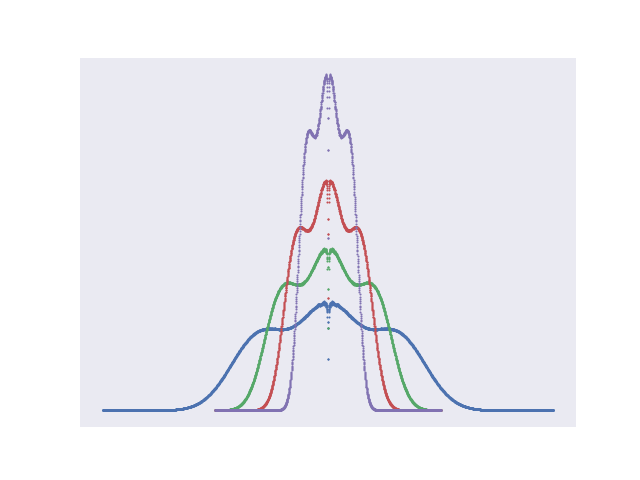
\includegraphics[scale=0.7]{Images/art.png}
	\caption{One-body density plots for a two-dimensional single quantum dot containing 12 electrons, popularly called an artificial Magnesium atom. The four graphs correspond to four different oscillator frequencies, where the weakest oscillator gives the broadest density distribution. It's quite artistic, isn't it?}
\end{figure}
After all, this thesis is related to a master in physics, and therefore the results and the physical insight is the interesting part. Before we move on to the physical results, we will take a quick look at some more technical results, more precisely the computational cost of various wave function structures and the energy convergence using various optimization tools. 

For validation purposes, we will present a few selected results on the case without repulsive interaction and compare to analytical results. Thereafter, we study the case with repulsive interaction in a much larger scale, where we compare various wave function structures for different number of particles and oscillator strengths in two and three dimensions.

\newpage
\section{Computational cost}
One of the major problems of simulating quantum many-body systems is the computational cost, which explodes as the system size increases. In figure \eqref{fig:cpu_time} the CPU-time is plotted as a function of number of particles. We observe that the restricted Boltzmann machine (RBM) generally is cheaper to calculate compared to standard variational Monte-Carlo (VMC), which is a bit surprising. In the VMC trial wave function, we have only two variational parameters, while we in the RBM have $D\cdot N \cdot (1+H)+H$ with $N$ as number of particles, $D$ as the number of dimensions and $H$ as the number of hidden nodes. Throughout this thesis, we always set $H=N$, which gives 10,584 parameters for 72 particles in two dimensions and 14,980 parameters for 70 particles in three dimensions. 

In other words, this evolve to be an optimization problem. The reason why the RBM still appears to have a cheaper cost, is probably that we do not need to calculate the distance matrix over and over again. For RBM+SJ and RBM+PJ, the cost is significantly higher due to the distance matrix.

\begin{figure} %[h]
	\centering
	% This file was created by matplotlib2tikz v0.7.4.
\begin{tikzpicture}[scale=0.9]

\begin{axis}[name=2D, xlabel=$N$, ylabel={CPU-time [s]}, grid=major, 
legend cell align={left},
legend style={at={(1.68,1.10)}, anchor=south east, draw=white!80.0!black},
legend columns = 6, 
clip=false,
xtick=data] 
\addplot[color=color0,mark=oplus*, dashed] coordinates { 
	(2,6.05)
	(6,11.25)
	(12,20.53) 
	(20,38.99) 
	(30,73.73) 
	(42,130.49) 
	(56,213.47)
	(72,360.22)
	(90,856.84) }; 
\addlegendentry{RBM};

\addplot[color=color1,mark=oplus*, dash dot] coordinates { 
	(2,7.12) 
	(6,14.07) 
	(12,28.42) 
	(20,63.27) 
	(30,122.93) 
	(42,199.60)
	(56,349.22)}; 
\addlegendentry{RBM+SJ};

\addplot[color=color2,mark=oplus*, dotted] coordinates { 
	(2,7.26)
	(6,13.50)
	(12,27.68)
	(20,57.09) 
	(30,119.17) 
	(42,212.53) 
	(56,382.13) }; 
\addlegendentry{RBM+PJ};

\addplot[color=color3,mark=oplus*] coordinates { 
	(2,5.11)
	(6,10.51)
	(12,20.85) 
	(20,41.20) 
	(30,76.26) 
	(42,137.39) 
	(56,230.63)
	(72,355.81)
	(90,544.03) }; 
\addlegendentry{VMC};

\node[] at (axis cs: 44,978) {2D};
\end{axis}

\begin{axis}[name=2D, 
xshift=7.9cm, 
xlabel=$N$, 
grid=major, 
clip=false,
xtick=data] 
\addplot[color=color0,mark=oplus*, dashed] coordinates { 
	(2,7.69)
	(8,20.92)
	(20,59.67) 
	(40,171.84) 
	(70,586.39) }; 
%\addlegendentry{RBM};

\addplot[color=color1,mark=oplus*, dash dot] coordinates { 
	(2,8.95)
	(8,26.86)
	(20,94.64) 
	(40,270.92) }; 
%\addlegendentry{RBM+SJ};

\addplot[color=color2,mark=oplus*, dotted] coordinates { 
	(2,8.87)
	(8,26.36)
	(20,91.40) 
	(40,293.25) }; 
%\addlegendentry{RBM+PJ};

\addplot[color=color3,mark=oplus*] coordinates { 
	(2,6.70)
	(8,20.99)
	(20,62.54) 
	(40,185.65) 
	(70,486.02) };
%\addlegendentry{VMC};

\node[] at (axis cs: 35,670) {3D};
\end{axis}
\end{tikzpicture}
	\label{fig:cpu_time}
	\caption{CPU-time per iteration as a function of number of particles for two and three dimensions. The solid line is standard variational Monte-Carlo (VMC), while the dashed lines are restricted Boltzmann machines without Jastrow factor (RBM), with simple Jastrow factor (RBM+SJ) and with Padé-Jastrow factor (RBM+PJ)}
\end{figure}

As the applied theory used in quantum many-body simulations agrees perfectly with laboratory experiments, they can be considered as actual experiments. In that manner, one can use computer experiments to verify other experiments and even predict new things. Similarly to experiments in a laboratory, computer experiments are also dependent on external factors, especially when it comes to the CPU-time, and therefore it is important to do such measurements multiple times to find an accurate average time. The CPU-times above are the average from at least four independent runs for each number of particles. All the runs were performed on the Abel computational cluster, which is equipped with Supermicro X9DRT compute nodes with dual Intel E5-2670 CPUs running at 2.6 GHz. Different hardware might give different CPU-times, but the CPU-time ratios (the exponential factor) should be the same. 

To estimate how fast the cost increases as we add more particles, we do linear regression with a function on the form $f(x)=\alpha x^{\beta}$ where $x$ is the number of particles while $\alpha$ and $\beta$ are the unknown parameters to be found. From the limited number of points, we have found the parameters and presented them in table \eqref{tab:cputimefit}.

\begin{table} [H]
	\caption{Optimal constants $\alpha$ and $\beta$ for restricted Boltzmann machine (RBM), restricted Boltzmann machine with a simple Jastrow factor (RBM+SJ), restricted Boltzmann machine with Padé-Jastrow factor (RBM+PJ) and standard variational Monte-Carlo sampling (VMC).}
	\begin{tabularx}{\textwidth}{X|CC:CC} \hline\hline
		\label{tab:cputimefit}
		& \multicolumn{2}{c}{2D} &
		\multicolumn{2}{c}{3D} \\ \hline
		& $\alpha$ & $\beta$ & $\alpha$ & $\beta$ \\ \hline \\
		RBM & 0.0840 & 1.92 & 0.0302 & 2.268 \\ 
		RBM+SJ & - & - & - & - \\
		RBM+PJ & - & - & - & - \\
		VMC & 0.111 & 1.88 & 0.148 & 1.91 \\ \hline\hline
	\end{tabularx}
\end{table}

Although the RBM was found to be cheaper than VMC, we can see that the estimated exponential factor $\alpha$ is actually slightly larger. The prefactor $\beta$ is significantly lower though.

\section{Energy convergence}
We want our calculations to converge fast and to be stable, and that is what the optimization tools are responsible for. In figure \eqref{fig:convergenceoptimization} we compare standard gradient descent to stochastic gradient descent and ADAM for two interacting electrons in a two- and three dimensional well. 

\begin{figure} [H]
	\centering
	\begin{tikzpicture} [scale=0.9, spy using outlines=
	{rectangle, magnification=8,size=2cm, height=1cm, connect spies}]
	\begin{axis} [name=2D, xlabel=Iteration, ylabel={Energy [Ha]}, grid=major, every axis plot/.append style={thick}]
		\addplot table [x expr=\coordindex+1, y index=0, mark=none] {/home/evenmn/VMC/data/int1/energy/VMC/2D/2P/1.000000w/GD_MC16777216.dat};
		\addlegendentry{GD};
		
		\addplot table [x expr=\coordindex+1, y index=0, mark=none, green] {/home/evenmn/VMC/data/int1/energy/VMC/2D/2P/1.000000w/ADAM_MC16777216.dat}; 
		\addlegendentry{ADAM};
		
		\addplot+ [dashed,mark=none,black] coordinates {(0,3) (100,3)};
		\addlegendentry{Exact};
		
		\coordinate (spypoint1) at (axis cs:75,2.995);
		\coordinate (magnifyglass1) at (axis cs:50,3.05);
	\end{axis}
	\spy [size=2.0cm] on (spypoint1)
	in node[fill=white] at (magnifyglass1);
	
	\begin{axis} [name=3D, at=(2D.right of south east), anchor=left of south west, xlabel=Iteration, grid=major, every axis plot/.append style={thick}]	
		\addplot table [x expr=\coordindex+1, y index=0, mark=none] {/home/evenmn/VMC/data/int1/energy/VMC/3D/2P/0.500000w/GD_MC16777216.dat};  
		\addlegendentry{GD};
		
		\addplot table [x expr=\coordindex+1, y index=0, mark=none] {/home/evenmn/VMC/data/int1/energy/VMC/3D/2P/0.500000w/ADAM_MC16777216.dat}; 
		\addlegendentry{ADAM};
		
		\addplot+ [dashed,mark=none,color=black] coordinates {(0,2) (100,2)};
		\addlegendentry{Exact};
		
		\coordinate (spypoint2) at (axis cs:75,1.997);
		\coordinate (magnifyglass2) at (axis cs:50,2.04);
	\end{axis} 
	\spy [size=2.0cm] on (spypoint2)
	in node[fill=white] at (magnifyglass2);
\end{tikzpicture}
	\caption{Energy convergence for circular quantum dots of two particles in two dimensions (left) and three dimensions (right). We use a standard variational Monte-Carlo wave function, the learning rate was set to $\eta=0.5$ and the number of Metropolis steps used for each iteration was $M=2^{24}=16,777,216$.}
\end{figure}

We observe that the gradient descent methods in the cases above have a smoother convergence compared ADAM. However, this could be the case for the standard variational Monte-Carlo wave function only, so we better also look how well they do for other structures. 
\iffalse
\begin{figure}[H]
	\centering
	\label{fig:convergenceoptimization2}
	\subfloat[2D, 2P, $\omega=1$]{{\includegraphics[width=8cm]{/home/evenmn/VMC/plots/int1/energy/2D/2P/1.000000w/MC2pow24.png}}}
	\subfloat[3D, 2P, $\omega=1/2$]{{\includegraphics[width=8cm]{/home/evenmn/VMC/plots/int1/energy/3D/2P/0.500000w/MC2pow24.png}}}
	\caption{Energy convergence for two electrons in a two dimensional (a) and three dimensional (b) quantum dot. The learning rate was set to $\eta=0.5$, and the number of Metropolis steps used for each iteration was $MC=2^{24}$.}
\end{figure}
\fi

\iffalse
\begin{figure}[H]
	\centering
	
\includegraphics[scale=0.3]{Images/example.png}
	\caption{Will add convergence plots here}
\end{figure}
\fi

Even though the gradient descent methods seem to be the best choice based on those graphs, we experience that the energy occasionally explode when they are applied on more heavy systems, and therefore we will rely in the ADAM optimizer henceforth. 

\newpage
\section{No repulsive interaction}
We start with the non-interacting case in order to validate the implemented code. In this case we both know the exact energies and the exact one-body densities for an array of systems, and can therefore validate the code.

\subsection{Quantum dots}
We will start with quantum dots, 

\subsubsection{Ground-state energy}
The single quantum dot has analytical ground-state energies given by equation \eqref{eq:HOenergies} and number of closed-shell particles given by equation \eqref{eq:HOclosedshell}. The first 5 closed-shell energies for $\omega=0.5$ and $\omega=1.0$ are presented in table \eqref{tab:quantumdotswointeraction}.

\begin{table}[H]
	\caption{Energy of circular quantum dots of frequency $\omega=0.5$ and $\omega=1.0$ consisting of $N$ non-interacting particles. RBM is a single Slater determinant with a plain Boltzmann machine baked in, while VMC is a standard variational Monte-Carlo Slater determinant. Exact values are obtained by $E=\omega(n+1/2)$, and all values are given in units of $\hbar$.}
	\label{tab:quantumdotswointeraction}
	\begin{tabularx}{\textwidth}{r|r|R{2cm}R{2cm}R{2cm}|R{2cm}R{2cm}R{2cm}} \hline\hline
		&& \multicolumn{3}{c}{$\omega=0.5$}&\multicolumn{3}{c}{$\omega=1.0$}\\ \hline
		\makecell{\\ \phantom{=}}& $N$ & \multicolumn{1}{c}{RBM} & \multicolumn{1}{c}{VMC} & \multicolumn{1}{c}{Exact} & \multicolumn{1}{c}{RBM} & \multicolumn{1}{c}{VMC} & \multicolumn{1}{c}{Exact} \\ \hline \\
		
		\parbox[t]{2mm}{\multirow{5}{*}{\rotatebox[origin=c]{90}{2D}}}
		&2 & 1.0 & 1.0 & 1 & 2.0 & 2.0 & 2\\
		&6 & 5.0 & 5.0 & 5 & 10.0 & 10.0 & 10 \\
		&12 & 14.0 & 14.0 & 14 & 28.0 & 28.0 & 28\\
		&20 & 30.0 & 30.0 & 30 & 60.0 & 60.0 & 60\\
		&30 & 55.0 & 55.0 & 55 & 110.0 & 110.0 & 110\\ \hline \\
		
		\parbox[t]{2mm}{\multirow{5}{*}{\rotatebox[origin=c]{90}{3D}}}
		&2 & 1.5 & 1.5 & 1.5 & 3.0 & 3.0 & 3 \\
		&8 & 9.0 & 9.0 & 9 & 18.0 & 18.0 & 18 \\
		&20 & 30.0 & 30.0 & 30 & 60.0 & 60.0 & 60 \\
		&40 & 75.0 & 75.0 & 75 & 150.0 & 150.0 & 150 \\
		&70 & 157.5 & 157.5 & 157.5 & 315.0 & 315.0 & 315 \\ \hline\hline
	\end{tabularx}
\end{table}
We observe that both the standard VMC, with $\alpha=1$, and standard RBM, with all parameters set to zero, are able to reproduce the analytical expression. 

\newpage
\subsubsection{One-body density}
We will also focus on the one-body densities throughout the results, and comparing the obtained densities to the analytical ones is a good indicator on whether the implementation is correct or not. In figure \eqref{fig:OB_nointeraction} the one-body densities are plotted for quantum dots of two non-interacting electrons. The analytical one-body densities are found from the definition of one-body density in equation \eqref{eq:electron_density}.

\begin{figure} [h]%
	\centering
	\subfloat[2D, $\omega=0.5$]{{\includegraphics[width=8cm]{/home/evenmn/VMC/plots/int0/onebody/2D/2P/GD_MC2pow28_w0p5.png}}}
	\subfloat[2D, $\omega=1.0$]{{\includegraphics[width=8cm]{/home/evenmn/VMC/plots/int0/onebody/2D/2P/GD_MC2pow28_w1p0.png} }}\\
	
	\subfloat[3D, $\omega=0.5$]{{\includegraphics[width=8cm]{/home/evenmn/VMC/plots/int0/onebody/3D/2P/GD_MC2pow28_w1p0.png} }}
	\subfloat[3D, $\omega=1.0$]{{\includegraphics[width=8cm]{/home/evenmn/VMC/plots/int0/onebody/3D/2P/GD_MC2pow28_w0p5.png} }}
	\caption{One-body densities of two non-interacting electrons in two- and three dimensions for $\omega=0.5$ and $\omega=1.0$.}%
	\label{fig:OB_nointeraction}
\end{figure}

We observe that both the standard variational Monte-Carlo wave function (VMC) and the restricted Boltzmann machine (RBM) reproduce the analytical one-body density. The distribution gets narrower as the frequency is increased, and we also observe that the distributions are identical for two- and three dimensions with the same frequency.

\newpage
\subsection{Atoms}
Also atoms will be studied as well...

\subsubsection{Ground-state energy}
\begin{table} [H]
	\caption{Energy of atoms of $N$ non-interacting electrons. RBM is a single Slater determinant with a plain Boltzmann machine baked in, while VMC is a standard variational Monte-Carlo Slater determinant.}
	\label{tab:atomswointeraction}
	\begin{tabularx}{\textwidth}{lrrR{3.5cm}R{3.5cm}R{3.5cm}} \hline\hline
		Atom & $N$ & \makecell{\\ \phantom{=}} & RBM & VMC & Exact \\ \hline \\
		
		H & 1 && - & -0.5 & -0.5 \\
		He & 2 && - & -4.0 & -4 \\
		Be & 4 && - & -20.0 & -20 \\
		Ne & 10 && - & -200.0 & -200\\
		Mg & 12 && - & - & -320 \\ \hline\hline
	\end{tabularx}
\end{table}

\newpage
\section{Quantum Dots}
We now move on to the more interesting case with repulsive interaction, where we no longer have analytical results, apart from a few semi-analytical energies and wave functions  for the two- and three-dimensional single quantum dots.

To achieve good results, we apply an adaptive step number, which means that the number of steps per iteration is increased for the last iterations. Firstly, this makes the final energy more accurate due to better statistics. Secondly, we get less noisy electron density plots by using this technique. All results below are produced using $2^{20}=1,048,576$ number of steps per iteration for the initial iterations. Then the number of steps is increased to $2^{24}=16,777,216$ when we have 11 iterations left, and for the very last iteration we use $2^{28}=268,435,456$ steps.

Initially we look at standard quantum dots of size up to $N=56$ electrons in 2D and $N=40$ electrons in 3D and frequencies between $\omega=1.0$ and $\omega=0.1$. For those systems, we will compute the ground state energy, the one-body density and the two-body density. 

After that, we move on to some special cases where the dots have low frequency ($\omega=0.01$), the total spin projection $S=\sum_im_s$ is unlike zero, the quantum dots are in a medium or the number of electrons is large. For those systems, we will typically focus on either the ground-state energy or the one-body density dependent on what we want to investigate. For instance, we will focus on the one-body density for low frequency dots because of the search for Wigner crystals. 

\subsection{Ground-state energy}
By utilizing the symmetry of quantum dots of two electrons, M.Taut was able to obtain semi-analytical energies for some specific frequencies $\omega$. More precisely, he found the energy to be $E=3$ for the frequency $\omega=1$ and $E=2/3$ for the frequency $\omega=1/6$ for the two-dimensional case, and $E=2$ for the frequency $\omega=1/2$ and $E=1/2$ for the frequency $\omega=1/10$ for the three-dimensional case. \cite{taut_two_1993}\cite{taut_two_1994}

For other references, we need to rely on what researchers have found before us. Since diffusion Monte-Carlo (DMC) is known to give very accurate results, we will mainly compare our results to J. Høgberget's DMC computations, which exist for closed shell quantum dots of a maximum of 56 electrons in two dimensions and a maximum of 20 particles in three dimensions. \cite{hogberget_quantum_2013}. Comparing the energy to the Hartree-Fock limit is also interesting, mainly because of the Boltzmann machines. We use A.Mariadason's computations for this for quantum dots of a maximum of 20 electrons in two dimensions, and a maximum of 8 particles in three dimensions. \cite{mariadason_quantum_2018}

Ground state energy computations of two- and three dimensional quantum dots are found in tables \eqref{tab:quantumdotswinteraction2D1} and \eqref{tab:quantumdotswinteraction3D1} respectively. They are performed by a restricted Boltzmann machine (RBM), restricted Boltzmann machine with a simple Jastrow factor (RBM+SJ), restricted Boltzmann machine with Padé-Jastrow factor (RBM+PJ), partly restricted Boltzmann machine (PRBM) and standard variational Monte-Carlo (VMC). In addition, the Hartree-Fock limit (HF) and diffusion Monte-Carlo (DMC) are present for reference purposes. 

We observe that the method where less physical intuition is used, RBM, is the one that gives the highest energies. However, compared to HF, the energy is mostly lower. When we add more intuition in form of a simple Jastrow factor, the energy drops significantly. RBM+PJ and VMC are on the same level, with VMC pinched in front.

\afterpage{
\begin{landscape}
\begin{table}
	\caption{The ground state energy of two-dimensional circular quantum dots of frequency $\omega$ obtained by various methods. The column on the left-hand-side represents restricted Boltzmann machine (RBM), followed by restricted Boltzmann machine with simple Jastrow factor (RBM+SJ), restricted Boltzmann machine with Padé-Jastrow factor (RBM+PJ), partly restricted Boltzmann machine (PRBM), the Hartree-Fock limit (HF), standard variational Monte-Carlo with Hartree-Fock basis (VMC+HF), standard variational Monte-Carlo with Hermite basis (VMC) and diffusion Monte-Carlo (DMC). Hartree-Fock results are taken from Ref.\cite{mariadason_quantum_2018}, DMC results are taken from \cite{hogberget_quantum_2013} and semi-analytical results are taken from \cite{taut_two_1994}. $N$ is the number of electrons in the dot, and $L=S=0$. The energy is given in units of $\hbar$, and the numbers in parenthesis are the statistical uncertainties in the last digit.}
	\begin{tabularx}{\hsize}{llR{2.3cm}R{2.3cm}R{2.3cm}R{2.3cm}R{2.3cm}R{2.3cm}R{2.3cm}R{2.3cm}} \hline\hline
		\label{tab:quantumdotswinteraction2D1}
		\makecell{\\ $N$ \\ \phantom{=}} & $\omega$ & \multicolumn{1}{c}{RBM} & \multicolumn{1}{c}{RBM+SJ} & \multicolumn{1}{c}{RBM+PJ} & \multicolumn{1}{c}{PRBM} & \multicolumn{1}{c}{\makecell{HF \\ (Ref.\cite{mariadason_quantum_2018})}} & \multicolumn{1}{c}{\makecell{VMC+HF \\ (Ref.\cite{mariadason_quantum_2018})}} & \multicolumn{1}{c}{VMC} & \multicolumn{1}{c}{\makecell{DMC \\ (Ref.\cite{hogberget_quantum_2013})}} \\ \hline \\
		2 & 0.1 & 0.4728(1) & 0.44859(6) & 0.440975(8) & 0.4959(2) & 0.525635 & - & 0.44129(1) & 0.44079(1) \\ 
		& 1/6 & 0.7036(1) & 0.67684(7) & 0.66715(6) & 0.7326(2) & 0.768675 & - & 0.66710(1) & $0.\bar{6}^{1}$ \\
		& 0.28 & 1.0707(2) & 1.03485(7) & 1.021668(7) & 1.0987(2) & 1.14171 & - & 1.02192(1) & 1.02164(1) \\
		& 0.5 & 1.7234(2) & 1.67787(8) & 1.659637(6) & 1.7182(3) & 1.79974 & - & 1.65974(1) & 1.65977(1)  \\
		& 1.0 & 3.0829(2) & 3.0255(1) & 2.999587(5) & 3.0566(3) & 3.16190 & - & 2.99999(1) & $3.0^{1}$ \\ \hdashline \\

		6 & 0.1 & 3.697(1) & 3.6584(4) & 3.57832(2) & - & 3.85238 & - & 3.5698(1) & 3.55385(5) \\ 
		& 0.28 & 7.9273(9) & 7.7503(4) & 7.6245(2) & - & 8.01957 & - & 7.6219(1) & 7.60019(6) \\
		& 0.5 & 12.241(1) & 11.9659(5) & 11.8113(2) & 11.995(3) & 12.2713 & - & 11.8104(2) & 11.78484(6) \\
		& 1.0 & 20.716(1) & 20.4061(7) & 20.1853(2) & 20.483(1) & 20.7192 & - & 20.1918(2) & 20.15932(8) \\ \hdashline \\
		
		12 & 0.1 & 12.705(2) & 12.566(2) & 12.3416(4) & - & 12.9247 & - & 12.3196(3) & 12.26984(8) \\ 
		& 0.28 & 26.389(2) & 26.083(1) & 25.7331(5) & - & 26.5500 & - & 25.7049(4) & 25.63577(9) \\
		& 0.5 & 40.440(3) & 39.694(1) & 39.2743(6) & - & 40.2161 & - & 39.2421(5) & 39.1596(1) \\
		& 1.0 & 67.632(3) & 66.378(2) & 65.9550(7) & - & 66.9113 & - & 65.7928(5) & 65.7001(1) \\ \hdashline
	\end{tabularx}
\end{table}

\begin{table}
	\begin{tabularx}{\hsize}{llR{2.3cm}R{2.3cm}R{2.3cm}R{2.3cm}R{2.3cm}R{2.3cm}R{2.3cm}R{2.3cm}} \\
		\label{tab:quantumdotswinteraction2D2}
		20 & 0.1 & 30.824(2) & 30.567(3) & 30.1553(9) & - & 31.1902 & - & 30.086(1) & 29.9779(1) \\ 
		& 0.28 & 63.746(4) & 62.811(3) & 62.148(1) & - & 63.5390 & - & 62.0755(7) & 61.9268(1) \\
		& 0.5 & 97.166(5) & 94.920(4) & 94.104(1) & - & 95.7328 & - & 94.0433(9) & 93.8752(1) \\
		& 1.0 & 159.640(5) & 157.209(4) & 156.104(1) & - & 158.004 & - & 156.102(1) & 155.8822(1) \\ \hdashline \\
		
		30 & 0.1 & 61.829(5) & 61.351(4) & 60.774(2) & - & - & - & 60.585(1) & 60.4205(2) \\ 
		& 0.28 & 126.958(6) & 126.067(5) & 124.437(2) & - & - & - & 124.195(2) & 123.9683(2) \\
		& 0.5 & 191.495(7) & 188.995(5) & 187.493(2) & - & - & - & 187.325(3) & 187.0426(2) \\
		& 1.0 & 315.364(8) & 311.468(7) & 308.989(2) & - & - & - & 308.957(2) & 308.5627(2) \\ \hdashline \\
		
		42 & 0.1 & 109.892(6) & 110.030(7) & - & - & - & - &  107.928(2) & 107.6389(2) \\ 
		& 0.28 & 224.462(8) & 224.587(8) & - & - & - & - & 220.224(2) & 219.8426(2) \\
		& 0.5 & 337.523(8) & 333.582(9) & 331.410(3) & - & - & - & 331.276(3) & 330.6306(2) \\
		& 1.0 & 553.40(1) & 549.76(1) & 543.746(3) & - & - & - & 543.738(7) & 542.9428(8) \\ \hdashline \\
		
		56 & 0.1 & - & 180.52(1) & - & - & - & - & 176.774(3) & 175.9553(7) \\ 
		& 0.28 & 364.85(1) & 366.91(1) & - & - & - & - & 359.63(1) & 358.145(2) \\
		& 0.5 & 547.46(1) & 545.74(1) & - & - & - & - & 538.686(9) & 537.353(2) \\
		& 1.0 & 894.12(2) & 890.70(2) & - & - & - & - & 880.352(5) & 879.3986(6) \\ \hline\hline
	\end{tabularx}
\end{table}

\begin{table}
	\caption{The ground state energy of three-dimensional circular quantum dots of frequency $\omega$ obtained by various methods. The column on the left-hand-side represents restricted Boltzmann machine (RBM), followed by restricted Boltzmann machine with simple Jastrow factor (RBM+SJ), restricted Boltzmann machine with Padé-Jastrow factor (RBM+PJ), partly restricted Boltzmann machine (PRBM), the Hartree-Fock limit (HF), standard variational Monte-Carlo with Hartree-Fock basis (VMC+HF), standard variational Monte-Carlo with Hermite basis (VMC) and diffusion Monte-Carlo (DMC). Hartree-Fock results are taken from Ref.\cite{mariadason_quantum_2018}, DMC results are taken from \cite{hogberget_quantum_2013} and semi-analytical results are taken from \cite{taut_two_1993}. $N$ is the number of electrons in the dot, and $L=S=0$. The energy is given in units of $\hbar$, and the numbers in parenthesis are the statistical uncertainties in the last digit.} 
	\begin{tabularx}{\hsize}{llR{2.3cm}R{2.3cm}R{2.3cm}R{2.3cm}R{2.3cm}R{2.3cm}R{2.3cm}R{2.3cm}} \hline\hline
		\label{tab:quantumdotswinteraction3D1}
		\makecell{\\ $N$ \\ \phantom{=}} & $\omega$ & \multicolumn{1}{c}{RBM} & \multicolumn{1}{c}{RBM+SJ} & \multicolumn{1}{c}{RBM+PJ} & \multicolumn{1}{c}{PRBM} & \multicolumn{1}{c}{\makecell{HF \\ (Ref.\cite{mariadason_quantum_2018})}} & \multicolumn{1}{c}{\makecell{VMC+HF \\ (Ref.\cite{mariadason_quantum_2018})}} & \multicolumn{1}{c}{VMC} & \multicolumn{1}{c}{\makecell{DMC \\ (Ref.\cite{hogberget_quantum_2013})}} \\ \hline \\
		2 & 0.1 & 0.5178(1) & 0.50225(3) & 0.50009(6) & - & 0.529065 & - & 0.50008(4) & $0.5^{1}$ \\
		& 0.28 & 1.2259(1) & 1.20471(4) & 1.20201(5) & - & 1.23722 & - & 1.20174(6) & 1.201725(2) \\
		& 0.5 & 2.0269(1) & 2.00374(4) & 2.00009(4) & - & 2.03851 & - & 2.00000(5) & $2.0^{1}$ \\
		& 1.0 & 3.7571(1) & 3.73559(4) & 3.73032(4) & - & 3.77157 & - & 3.73002(5) & 3.730123(3) \\ \hdashline \\
		
		8 & 0.1 & 6.549(7) & 5.7995(5) & 5.8448(7) & - & 5.86255 & - & 5.7127(1) & 5.7028(1) \\ 
		& 0.28 & 13.098(2) & 12.2512(4) & 12.2054(2) & - & 12.3987 & - & 12.2051(1) & 12.1927(1) \\
		& 0.5 & 19.487(2) & 19.0266(4) & 18.9747(2) & - & 19.1916 & - & 18.9759(1) & 18.9611(1) \\
		& 1.0 & 33.302(1) & 32.739(4) & 32.6828(2) & - & 32.9246 & - & 32.6823(2) & 32.6680(1) \\ \hdashline \\
		
		20 & 0.1 & 27.813(2) & - & 29.425(9) & - & - & - & 27.3144(5) & 27.2717(2) \\ 
		& 0.28 & 57.700(4) & - & - & - & - & - & 56.4297(5) & 56.3868(2) \\
		& 0.5 & 87.840(4) & - & - & - & - & - & 85.7161(5) & 85.6555(2) \\
		& 1.0 & 146.292(4) & - & - & - & - & - & 142.9560(7) & 142.8875(2) \\ \hdashline \\
		
		40 & 0.1 & - & - & - & - & - & - & 88.182(1) & - \\ 
		& 0.28 & 182.714(6) & - & - & - & - & - & 179.567(1) & - \\
		& 0.5 & 275.262(7) & - & - & - & - & - & 269.746(1) & - \\
		& 1.0 & 452.732(8) & - & - & - & - & - & 442.602(2) & - \\ \hline\hline
	\end{tabularx}
\end{table}
\end{landscape}
}

\subsection{One-body density}
Another quantity of particular interest is the one-body density. We have produced one-body density plots using a restricted Boltzmann machine (RBM), a restricted Boltzmann machine with simple Jastrow factor (RBM+SJ), a restricted Boltzmann machine with Padé-Jastrow factor (RBM+PJ) and standard variational Monte-Carlo (VMC) for frequencies $\omega=[1.0,0.5,0.1]$ and up to 42 electrons in two dimensions and 40 electrons in three dimensions. The plots for two- and three-dimensional dots can be found in figures (\ref{fig:OB_interaction_2D_1w}-\ref{fig:OB_interaction_2D_01w}) and \ref{fig:OB_interaction_3D} respectively.

We observe that the density gets a wave shape with more peaks as the number of particles increases. The plain RBM tends to exaggerate the wave form, especially when the frequency gets lower, which is due to the lack of a Jastrow factor. The interaction gets more dominating as the frequency decreases, and the presence of Jastrow factor to handle the interactions is then important. We also see that the Padé-Jastrow factor works better than the simple Jastrow factor in all cases as expected.

\begin{figure} [H]
	\centering
	\subfloat[2P, $\omega=1.0$]{{\includegraphics[width=8cm]{/home/evenmn/VMC/plots/int1/onebody/2D/2P/1.000000w/ADAM_MC2pow28.png}}}
	\subfloat[6P, $\omega=1.0$]{{\includegraphics[width=8cm]{/home/evenmn/VMC/plots/int1/onebody/2D/6P/1.000000w/ADAM_MC2pow28.png}}}\\
	
	\subfloat[12P, $\omega=1.0$]{{\includegraphics[width=8cm]{/home/evenmn/VMC/plots/int1/onebody/2D/12P/1.000000w/ADAM_MC2pow28.png}}}
	\subfloat[20P, $\omega=1.0$]{{\includegraphics[width=8cm]{/home/evenmn/VMC/plots/int1/onebody/2D/20P/1.000000w/ADAM_MC2pow28.png}}}\\
	
	\subfloat[30P, $\omega=1.0$]{{\includegraphics[width=8cm]{/home/evenmn/VMC/plots/int1/onebody/2D/30P/1.000000w/ADAM_MC2pow28.png}}}
	\subfloat[42P, $\omega=1.0$]{{\includegraphics[width=8cm]{/home/evenmn/VMC/plots/int1/onebody/2D/42P/1.000000w/ADAM_MC2pow28.png}}}
	
	\caption{One-body density plots for two-dimensional circular quantum dots of 2, 6, 12, 20, 30 and 42 interacting electrons for frequencies $\omega=1.0$ produced by standard variational Monte-Carlo (VMC), plain restricted Boltzmann machine (RBM), restricted Boltzmann machine with simple Jastrow factor (RBM+SJ) and restricted Boltzmann machine with Padé-Jastrow factor (RBM+PJ). ADAM optimizer was used, and after convergence the number of Monte-Carlo cycles was $MC=2^{28}=268,435,456$.}
	\label{fig:OB_interaction_2D_1w}
\end{figure}
\begin{figure} [H]%
	\centering
	\subfloat[2P, $\omega=0.5$]{{\includegraphics[width=8cm]{/home/evenmn/VMC/plots/int1/onebody/2D/2P/0.500000w/ADAM_MC2pow28.png}}}
	\subfloat[6P, $\omega=0.5$]{{\includegraphics[width=8cm]{/home/evenmn/VMC/plots/int1/onebody/2D/6P/0.500000w/ADAM_MC2pow28.png}}}\\
	
	\subfloat[12P, $\omega=0.5$]{{\includegraphics[width=8cm]{/home/evenmn/VMC/plots/int1/onebody/2D/12P/0.500000w/ADAM_MC2pow28.png}}}
	\subfloat[20P, $\omega=0.5$]{{\includegraphics[width=8cm]{/home/evenmn/VMC/plots/int1/onebody/2D/20P/0.500000w/ADAM_MC2pow28.png}}}\\
	
	\subfloat[30P, $\omega=0.5$]{{\includegraphics[width=8cm]{/home/evenmn/VMC/plots/int1/onebody/2D/30P/0.500000w/ADAM_MC2pow28.png}}}
	\subfloat[42P, $\omega=0.5$]{{\includegraphics[width=8cm]{/home/evenmn/VMC/plots/int1/onebody/2D/42P/0.500000w/ADAM_MC2pow28.png}}}
	
	\caption{One-body density plots for two-dimensional circular quantum dots of 2, 6, 12, 20, 30 and 42 interacting electrons for frequencies $\omega=0.5$ produced by standard variational Monte-Carlo (VMC), plain restricted Boltzmann machine (RBM), restricted Boltzmann machine with simple Jastrow factor (RBM+SJ) and restricted Boltzmann machine with Padé-Jastrow factor (RBM+PJ). ADAM optimizer was used, and after convergence the number of Monte-Carlo cycles was $MC=2^{28}=268,435,456$.}%
	\label{fig:OB_interaction_2D_05w}
\end{figure}

\begin{figure} [H]%
	\centering
	\subfloat[2P, $\omega=0.1$]{{\includegraphics[width=8cm]{/home/evenmn/VMC/plots/int1/onebody/2D/2P/0.100000w/ADAM_MC2pow28.png}}}
	\subfloat[6P, $\omega=0.1$]{{\includegraphics[width=8cm]{/home/evenmn/VMC/plots/int1/onebody/2D/6P/0.100000w/ADAM_MC2pow28.png}}}\\
	
	\subfloat[12P, $\omega=0.1$]{{\includegraphics[width=8cm]{/home/evenmn/VMC/plots/int1/onebody/2D/12P/0.100000w/ADAM_MC2pow28.png}}}
	\subfloat[20P, $\omega=0.1$]{{\includegraphics[width=8cm]{/home/evenmn/VMC/plots/int1/onebody/2D/20P/0.100000w/ADAM_MC2pow28.png}}}\\
	
	\subfloat[30P, $\omega=0.1$]{{\includegraphics[width=8cm]{/home/evenmn/VMC/plots/int1/onebody/2D/30P/0.100000w/ADAM_MC2pow28.png}}}
	\subfloat[42P, $\omega=0.1$]{{\includegraphics[width=8cm]{/home/evenmn/VMC/plots/int1/onebody/2D/42P/0.100000w/ADAM_MC2pow28.png}}}
	
	\caption{One-body density plots for two-dimensional circular quantum dots of 2, 6, 12, 20, 30 and 42 interacting electrons for frequencies $\omega=0.1$ produced by standard variational Monte-Carlo (VMC), plain restricted Boltzmann machine (RBM), restricted Boltzmann machine with simple Jastrow factor (RBM+SJ) and restricted Boltzmann machine with Padé-Jastrow factor (RBM+PJ). ADAM optimizer was used, and after convergence the number of Monte-Carlo cycles was $MC=2^{28}=268,435,456$.}%
	\label{fig:OB_interaction_2D_01w}
\end{figure}
\begin{figure} [H]%
	\centering
	\subfloat[2P, $\omega=0.1$]{{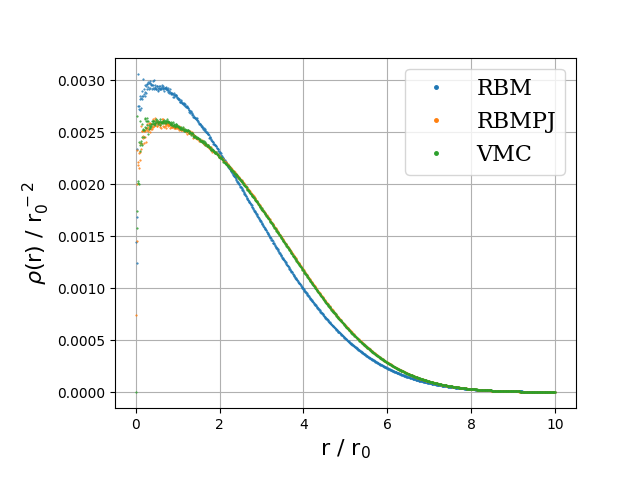
\includegraphics[width=8cm]{/home/evenmn/VMC/plots/int1/onebody/3D/2P/0.100000w/3D_2P_0p100000w_MC2pow28.png}}}
	\subfloat[8P, $\omega=0.1$]{{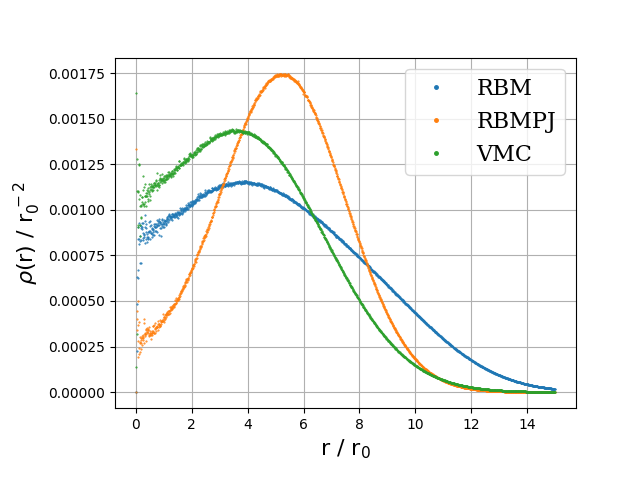
\includegraphics[width=8cm]{/home/evenmn/VMC/plots/int1/onebody/3D/8P/0.100000w/3D_8P_0p100000w_MC2pow28.png}}}\\
	
	\subfloat[2P, $\omega=0.5$]{{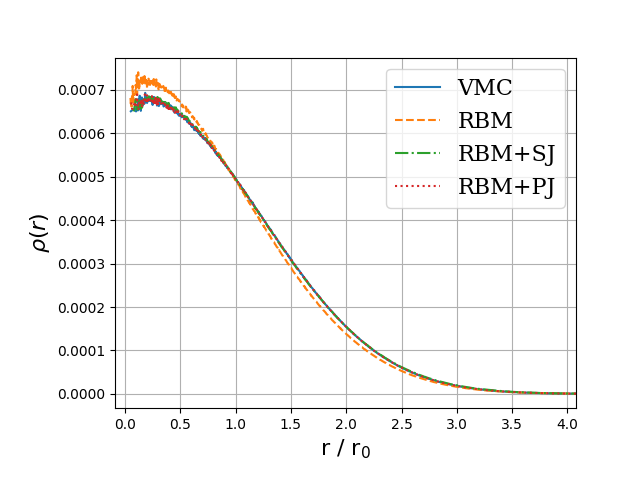
\includegraphics[width=8cm]{/home/evenmn/VMC/plots/int1/onebody/3D/2P/0.500000w/3D_2P_0p500000w_MC2pow28.png}}}
	\subfloat[8P, $\omega=0.5$]{{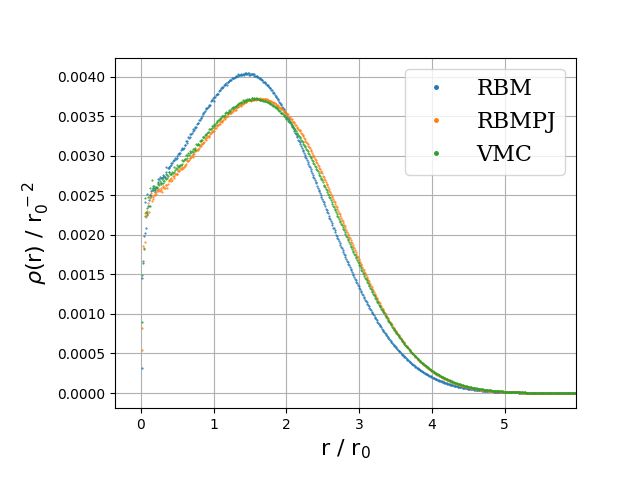
\includegraphics[width=8cm]{/home/evenmn/VMC/plots/int1/onebody/3D/8P/0.500000w/3D_8P_0p500000w_MC2pow28.png}}}\\
	
	\subfloat[2P, $\omega=1.0$]{{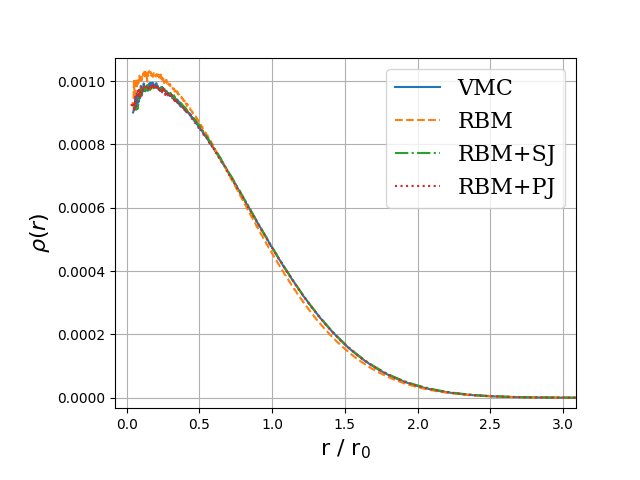
\includegraphics[width=8cm]{/home/evenmn/VMC/plots/int1/onebody/3D/2P/1.000000w/3D_2P_1p000000w_MC2pow28.png}}}
	\subfloat[8P, $\omega=1.0$]{{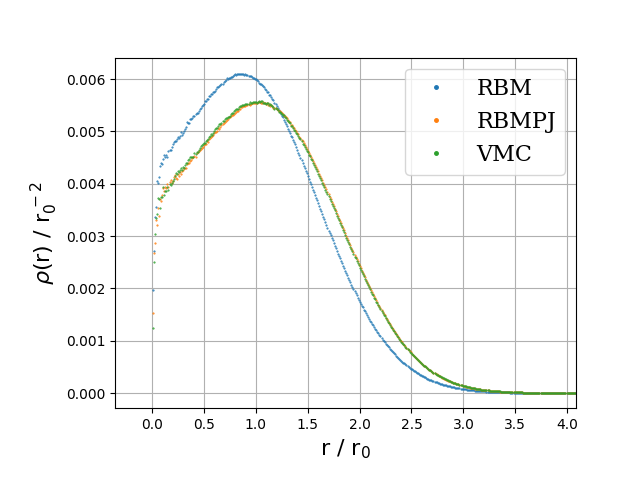
\includegraphics[width=8cm]{/home/evenmn/VMC/plots/int1/onebody/3D/8P/1.000000w/3D_8P_1p000000w_MC2pow28.png}}}
	
	%\caption{One-body densities of two and eight interacting electrons in three dimensions for various oscillator frequencies produced by standard variational Monte-Carlo (VMC), plain restricted Boltzmann machine (RBM) and restricted Boltzmann machine with Padé-Jastrow factor (RBMPJ). Stochastic gradient descent was used, and after convergence the number of Monte-Carlo cycles was $MC=2^{28}=268.435.456$.}%
	%\label{fig:OB_interaction_2P_3D}
\end{figure}
\begin{figure} [H]%
	\centering
	\subfloat[2P, $\omega=0.1$]{{\includegraphics[width=8cm]{/home/evenmn/VMC/plots/int1/onebody/3D/20P/0.100000w/ADAM_MC2pow28.png}}}
	\subfloat[8P, $\omega=0.1$]{{\includegraphics[width=8cm]{/home/evenmn/VMC/plots/int1/onebody/3D/40P/0.100000w/ADAM_MC2pow28.png}}}\\
	
	\subfloat[2P, $\omega=0.5$]{{\includegraphics[width=8cm]{/home/evenmn/VMC/plots/int1/onebody/3D/20P/0.500000w/ADAM_MC2pow28.png}}}
	\subfloat[8P, $\omega=0.5$]{{\includegraphics[width=8cm]{/home/evenmn/VMC/plots/int1/onebody/3D/40P/0.500000w/ADAM_MC2pow28.png}}}\\
	
	\subfloat[2P, $\omega=1.0$]{{\includegraphics[width=8cm]{/home/evenmn/VMC/plots/int1/onebody/3D/20P/1.000000w/ADAM_MC2pow28.png}}}
	\subfloat[8P, $\omega=1.0$]{{\includegraphics[width=8cm]{/home/evenmn/VMC/plots/int1/onebody/3D/40P/1.000000w/ADAM_MC2pow28.png}}}
	
	\caption{One-body density plots for three-dimensional circular quantum dots of 2, 8, 20 and 40 interacting electrons for various oscillator frequencies $\omega$ produced by standard variational Monte-Carlo (VMC), plain restricted Boltzmann machine (RBM), restricted Boltzmann machine with simple Jastrow factor (RBM+SJ) and restricted Boltzmann machine with Padé-Jastrow factor (RBM+PJ). ADAM optimizer was used, and after convergence the number of Monte-Carlo cycles was $MC=2^{28}=268,435,456$.}%
	\label{fig:OB_interaction_3D}
\end{figure}

\subsection{Two-body density}
The last thing we will investigate, is the two-body density. See figure \eqref{fig:TB_interaction_2D}.

\begin{landscape}
	\begin{figure} [H]%
		\centering
		\subfloat[RBM, 2P]{{\includegraphics[width=5cm]{/home/evenmn/VMC/plots/int1/twobody/2D/2P/1.000000w/RBM_ADAM_MC2pow28.png}}}
		\subfloat[RBM+SJ, 2P]{{\includegraphics[width=5cm]{/home/evenmn/VMC/plots/int1/twobody/2D/2P/1.000000w/RBMSJ_ADAM_MC2pow28.png}}}
		\subfloat[RBM+PJ, 2P]{{\includegraphics[width=5cm]{/home/evenmn/VMC/plots/int1/twobody/2D/2P/1.000000w/RBMPJ_ADAM_MC2pow28.png}}}
		\subfloat[VMC, 2P]{{\includegraphics[width=5cm]{/home/evenmn/VMC/plots/int1/twobody/2D/2P/1.000000w/VMC_ADAM_MC2pow28.png}}}\\
		
		\subfloat[RBM, 6P]{{\includegraphics[width=5cm]{/home/evenmn/VMC/plots/int1/twobody/2D/6P/1.000000w/RBM_ADAM_MC2pow28.png}}}
		\subfloat[RBM+SJ, 6P]{{\includegraphics[width=5cm]{/home/evenmn/VMC/plots/int1/twobody/2D/6P/1.000000w/RBMSJ_ADAM_MC2pow28.png}}}
		\subfloat[RBM+PJ, 6P]{{\includegraphics[width=5cm]{/home/evenmn/VMC/plots/int1/twobody/2D/6P/1.000000w/RBMPJ_ADAM_MC2pow28.png}}}
		\subfloat[VMC, 6P]{{\includegraphics[width=5cm]{/home/evenmn/VMC/plots/int1/twobody/2D/6P/1.000000w/VMC_ADAM_MC2pow28.png}}}\\
		
		\subfloat[RBM, 12P]{{\includegraphics[width=5cm]{/home/evenmn/VMC/plots/int1/twobody/2D/12P/1.000000w/RBM_ADAM_MC2pow28.png}}}
		\subfloat[RBM+SJ, 12P]{{\includegraphics[width=5cm]{/home/evenmn/VMC/plots/int1/twobody/2D/12P/1.000000w/RBMSJ_ADAM_MC2pow28.png}}}
		\subfloat[RBM+PJ, 12P]{{\includegraphics[width=5cm]{/home/evenmn/VMC/plots/int1/twobody/2D/12P/1.000000w/RBMPJ_ADAM_MC2pow28.png}}}
		\subfloat[VMC, 12P]{{\includegraphics[width=5cm]{/home/evenmn/VMC/plots/int1/twobody/2D/12P/1.000000w/VMC_ADAM_MC2pow28.png}}}\\
		
		%\caption{Two-body densities for interacting electrons in two dimensions for $\omega=0.5$ produced by standard variational Monte-Carlo (VMC), plain restricted Boltzmann machine (RBM) and restricted Boltzmann machine with Padé-Jastrow factor (RBMPJ). ADAM optimizer was used, and after convergence the number of Monte-Carlo cycles was $MC=2^{28}=268.435.456$.}%
		%\label{fig:TB_interaction_2D_1}
	\end{figure}
	
	\begin{figure} [H]%
		\centering
		\subfloat[RBM, 20P]{{\includegraphics[width=5cm]{/home/evenmn/VMC/plots/int1/twobody/2D/20P/1.000000w/RBM_ADAM_MC2pow28.png}}}
		\subfloat[RBM+SJ, 20P]{{\includegraphics[width=5cm]{/home/evenmn/VMC/plots/int1/twobody/2D/20P/1.000000w/RBMSJ_ADAM_MC2pow28.png}}}
		\subfloat[RBM+PJ, 20P]{{\includegraphics[width=5cm]{/home/evenmn/VMC/plots/int1/twobody/2D/20P/1.000000w/RBMPJ_ADAM_MC2pow28.png}}}
		\subfloat[VMC, 20P]{{\includegraphics[width=5cm]{/home/evenmn/VMC/plots/int1/twobody/2D/20P/1.000000w/VMC_ADAM_MC2pow28.png}}}
		
		\subfloat[RBM, 30P]{{\includegraphics[width=5cm]{/home/evenmn/VMC/plots/int1/twobody/2D/30P/1.000000w/RBM_ADAM_MC2pow28.png}}}
		\subfloat[RBM+SJ, 30P]{{\includegraphics[width=5cm]{/home/evenmn/VMC/plots/int1/twobody/2D/30P/1.000000w/RBMSJ_ADAM_MC2pow28.png}}}
		\subfloat[RBM+PJ, 30P]{{\includegraphics[width=5cm]{/home/evenmn/VMC/plots/int1/twobody/2D/30P/1.000000w/RBMPJ_ADAM_MC2pow28.png}}}
		%\subfloat[RBM+PJ, 30P]{{\includegraphics[width=4cm]{Images/example.png}}}
		\subfloat[VMC, 30P]{{\includegraphics[width=5cm]{/home/evenmn/VMC/plots/int1/twobody/2D/30P/1.000000w/VMC_ADAM_MC2pow28.png}}}\\
		
		\subfloat[RBM, 42P]{{\includegraphics[width=5cm]{/home/evenmn/VMC/plots/int1/twobody/2D/42P/1.000000w/RBM_ADAM_MC2pow28.png}}}
		\subfloat[RBM+SJ, 42P]{{\includegraphics[width=5cm]{/home/evenmn/VMC/plots/int1/twobody/2D/42P/1.000000w/RBMSJ_ADAM_MC2pow28.png}}}
		\subfloat[RBM+PJ, 42P]{{\includegraphics[width=5cm]{/home/evenmn/VMC/plots/int1/twobody/2D/42P/1.000000w/RBMPJ_ADAM_MC2pow28.png}}}
		\subfloat[VMC, 42P]{{\includegraphics[width=5cm]{/home/evenmn/VMC/plots/int1/twobody/2D/42P/1.000000w/VMC_ADAM_MC2pow28.png}}}\\
		
		\caption{Two-body densities for two-dimensional circular quantum dots of oscillator frequency $\omega=1.0$ produced with plain restricted Boltzmann machine (RBM), restricted Boltzmann machine with simple Jastrow factor (RBM+SJ), restricted Boltzmann machine with Padé-Jastrow factor (RBM+PJ) and standard variational Monte-Carlo (VMC). ADAM optimizer was used, and after convergence the number of Monte-Carlo cycles was $MC=2^{28}=268.435.456$.}%
		\label{fig:TB_interaction_2D}
	\end{figure}
\end{landscape}

\subsection{Splitting the energy}
It is also interesting to investigate how the energy is distributed between kinetic energy, external energy and interaction energy. 
\begin{table}
	\caption{Total energy ($\langle \hat{\mathcal{H}}\rangle$), kinetic energy ($\langle \hat{\mathcal{T}}\rangle$) and potential energy ($\langle \hat{\mathcal{V}}\rangle$) of circular quantum dots at a wide range of frequencies $\omega$. A standard variational Monte-Carlo wave function is used. The energy is given in units of $\hbar$, and the numbers in parenthesis are the statistical uncertainties in the last digit.}
	\label{tab:splitfrequencyQDVMC}
	\begin{tabularx}{\textwidth}{R{1.5cm}rrcR{2.3cm}R{2.3cm}R{2.3cm}R{2.3cm}} \hline\hline
		&\makecell{\\ $N$ \\ \phantom{=}} & $\omega$ && \multicolumn{1}{c}{$\langle \hat{\mathcal{H}}\rangle$} & \multicolumn{1}{c}{$\langle \mathcal{\hat{T}} \rangle$} & \multicolumn{1}{c}{$\langle \mathcal{\hat{V}_{\text{ext}}} \rangle$} & \multicolumn{1}{c}{$\langle \mathcal{\hat{V}_{\text{int}}} \rangle$} \\ \hline \\
		&2 & 0.01 && 0.074070(8) & 0.00947(3) & 0.02732(5) & 0.03728(4) \\
		&& 0.1 && 0.44129(1) & 0.09117(9) & 0.1789(1) & 0.17119(9) \\
		&& 0.28 && 1.02192(1) & 0.2477(1) & 0.4256(2) & 0.3487(1) \\
		&& 0.5 && 1.65974(1) & 0.4346(2) & 0.7057(2) & 0.5195(2)\\
		&& 1.0 && 2.99936(1) & 0.8523(3) & 1.3149(3) & 0.8321(2)\\
		&& 3.0 && 7.881906(9) & 2.5028(5) & 3.6911(6) & 1.6880(3) \\ \hdashline \\
		
		&6 & 0.01 && 0.6982(1) & 0.02735(7) & 0.2427(3) & 0.4281(3) \\
		&& 0.1 && 3.59(2) & 0.34(1) & 1.281(2) & 1.969(8) \\
		&& 0.28 && 7.6219(1) & 0.9105(4) & 2.8821(9) & 3.8292(7) \\
		&& 0.5 && 11.8104(2) & 1.6710(7) & 4.535(1) & 5.6045(9)\\
		&& 1.0 && 20.1918(2) & 3.405(1) & 8.046(1) & 8.741(1)\\
		&& 3.0 && \\ \hdashline \\
		
		&12 & 0.01 && 2.4972(3) & 0.05506(2) & 0.858(1) & 1.584(1)\\
		&& 0.1 && 12.3196(3) & 0.6885(6) & 4.393(2) & 7.238(2) \\
		&& 0.28 && 25.7049(4) & 2.090(1) & 9.355(2) & 14.260(2) \\
		&& 0.5 && 39.2421(5) & 3.939(2) & 14.564(3) & 20.739(3) \\
		&& 1.0 && 65.7928(5) & 8.536(3) & 24.874(4) & 32.383(3) \\
		&& 3.0 && 155.5235(1) & 23(1) & 63(1) & 68.4(2) \\ \hdashline \\
		
		&20 & 0.01 && 6.342(1) & 0.0559(2) & 2.125(6) & 4.161(6) \\
		&& 0.1 && 30.086(1) & 1.243(1) & 10.587(4) & 18.257(4) \\
		&& 0.28 && 62.0755(7) & 3.902(2) & 22.228(5) & 35.946(4) \\
		&& 0.5 && 94.0433(9) & 7.823(3) & 33.938(6) & 52.282(5) \\
		&& 1.0 && 156.102(1) & 16.86(1) & 58.14(1) & 81.098(6) \\
		&& 3.0 && 357.1(3) & 6(15) & 194(15) & 156.751(9) \\ \hline \hline
	\end{tabularx}
\end{table} 

\begin{table}
	\caption{Total energy ($\langle \hat{\mathcal{H}}\rangle$), kinetic energy ($\langle \hat{\mathcal{T}}\rangle$) and potential energy ($\langle \hat{\mathcal{V}}\rangle$) of circular quantum dots at a wide range of frequencies $\omega$. A standard restricted Boltzmann machine wave function is used. The energy is given in units of $\hbar$, and the numbers in parenthesis are the statistical uncertainties in the last digit.}
	\label{tab:splitfrequencyQDRBM}
	\begin{tabularx}{\textwidth}{R{1.5cm}rrcR{2.3cm}R{2.3cm}R{2.3cm}R{2.3cm}} \hline\hline
		&\makecell{\\ $N$ \\ \phantom{=}} & $\omega$ && \multicolumn{1}{c}{$\langle \hat{\mathcal{H}}\rangle$} & \multicolumn{1}{c}{$\langle \mathcal{\hat{T}} \rangle$} & \multicolumn{1}{c}{$\langle \mathcal{\hat{V}_{\text{ext}}} \rangle$} & \multicolumn{1}{c}{$\langle \mathcal{\hat{V}_{\text{int}}} \rangle$} \\ \hline \\
		&2 & 0.01 && - & - & - & - \\
		&& 0.1 && 0.473(3) & -0.05(3) & 0.35(3) & 0.178(4) \\
		&& 0.28 && 1.0707(2) & 0.2047(1) & 0.4678(3) & 0.3983(3) \\
		&& 0.5 && 1.7234(2) & 0.3739(2) & 0.7611(3) & 0.5884(3)\\
		&& 1.0 && 3.0829(2) & 0.7691(2) & 1.3926(4) & 0.9212(3)\\
		&& 3.0 && 7.9968(4) & 2.2346(5) & 4.0201(7) & 1.7422(4) \\ \hdashline \\
		
		&6 & 0.01 && 1.12(3) & -0.19(2) & 0.96(1) & 0.35(3) \\
		&& 0.1 && 3.77(1) & -0.11(3) & 2.04(4) & 2.04(4) \\
		&& 0.28 && 7.9273(9) & 0.8684(6) & 3.009(1) & 4.050(2) \\
		&& 0.5 && 12.241(1) & 1.611(1) & 4.709(2) & 5.921(2)\\
		&& 1.0 && 20.716(1) & 3.391(1) & 7.914(3) & 9.411(2)\\
		&& 3.0 && 49.415(1) & 10.309(3) & 21.456(4) & 17.649(2) \\ \hdashline \\
		
		&12 & 0.01 && - & - & - & - \\
		&& 0.1 && - & - & - & - \\
		&& 0.28 && - & - & - & - \\
		&& 0.5 && - & - & - & - \\
		&& 1.0 && - & - & - & - \\
		&& 3.0 && - & - & - & - \\ \hdashline \\
		
		&20 & 0.01 && - & - & - & - \\
		&& 0.1 && - & - & - & - \\
		&& 0.28 && - & - & - & - \\
		&& 0.5 && - & - & - & - \\
		&& 1.0 && - & - & - & - \\
		&& 3.0 && - & - & - & - \\ \hline \hline
	\end{tabularx}
\end{table} 

\begin{table}
	\caption{Total energy ($\langle \hat{\mathcal{H}}\rangle$), kinetic energy ($\langle \hat{\mathcal{T}}\rangle$) and potential energy ($\langle \hat{\mathcal{V}}\rangle$) of circular quantum dots at a wide range of frequencies $\omega$. A restricted Boltzmann machine with Padé-Jastrow wave function is used. The energy is given in units of $\hbar$, and the numbers in parenthesis are the statistical uncertainties in the last digit.}
	\label{tab:splitfrequencyQDRBMPJ}
	\begin{tabularx}{\textwidth}{R{1.5cm}rrcR{2.3cm}R{2.3cm}R{2.3cm}R{2.3cm}} \hline\hline
		&\makecell{\\ $N$ \\ \phantom{=}} & $\omega$ && \multicolumn{1}{c}{$\langle \hat{\mathcal{H}}\rangle$} & \multicolumn{1}{c}{$\langle \mathcal{\hat{T}} \rangle$} & \multicolumn{1}{c}{$\langle \mathcal{\hat{V}_{\text{ext}}} \rangle$} & \multicolumn{1}{c}{$\langle \mathcal{\hat{V}_{\text{int}}} \rangle$} \\ \hline \\
		&2 & 0.01 && - & - & - & - \\
		&& 0.1 && 0.440975(8) & 0.09223(9) & 0.1757(1) & 0.17304(9) \\
		&& 0.28 && 1.021668(7) & 0.2468(1) & 0.4258(2) & 0.3490(1) \\
		&& 0.5 && 1.659637(6) & 0.4305(2) & 0.7112(2) & 0.5179(2)\\
		&& 1.0 && 2.999587(5) & 0.8440(3) & 1.3418(3) & 0.8238(2)\\
		&& 3.0 && 7.882355(8) & 2.2466(6) & 4.0117(6) & 1.6240(3) \\ \hdashline \\
		
		&6 & 0.01 && - & - & - & - \\
		&& 0.1 && 17.13(3) & 0.4(1) & 16.2(1) & 0.531(5) \\
		&& 0.28 && - & - & - & - \\
		&& 0.5 && 11.8074(2) & 1.7018(7) & 4.513(1) & 5.5927(9) \\
		&& 1.0 && 20.1832(1) & 3.428(1) & 8.068(1) & 8.687(1) \\
		&& 3.0 && - & - & - & - \\ \hdashline \\
		
		&12 & 0.01 && 2.547(7) & 0.045(7) & 0.99(1) & 1.51(1) \\
		&& 0.1 && 16.52(2) & 0.71(2) & 11.28(2) & 4.529(6) \\
		&& 0.28 && 31.520(2) & 2.239(1) & 19.905(4) & 9.376(1) \\
		&& 0.5 && - & - & - & - \\
		&& 1.0 && 65.9578(7) & 8.240(2) & 26.931(4) & 30.787(3) \\
		&& 3.0 && 156.280(2) & 21.4(3) & 78.2(3) & 56.662(4) \\ \hdashline \\
		
		&20 & 0.01 && - & - & - & - \\
		&& 0.1 && - & - & - & - \\
		&& 0.28 && - & - & - & - \\
		&& 0.5 && - & - & - & - \\
		&& 1.0 && - & - & - & - \\
		&& 3.0 && - & - & - & - \\ \hline \hline
	\end{tabularx}
\end{table} 

\subsection{Low frequency dots}
When we lower the frequency, the potential energy dominates the kinetic energy. An evidence of that can be seen in table \eqref{tab:lowfrequencyQD}, where we present the expectation value of the total energy ($\langle \hat{\mathcal{H}}\rangle$) together with the expectation value of the kinetic energy ($\langle \hat{\mathcal{T}}\rangle$) and the expectation value of the potential energies ($\langle \mathcal{\hat{V}_{\text{ext}}} \rangle$,$\langle \mathcal{\hat{V}_{\text{int}}} \rangle$). From this, we can also see that the virial theorem, discussed in section \ref{sec:virial}, is satisfied.

As discussed in section \ref{sec:wigner}, at low kinetic energy the interaction is dominating, and in order to minimize this the electrons tend to orientate such that they maximize the distance to each other. They then form a lattice, known as Wigner crystals, and as we also claimed, this might be observed in the electron density plots. The one-body density of ...

\begin{figure}[H]
	\centering
	\includegraphics[scale=0.7]{/home/evenmn/VMC/plots/int1/onebody/2D/2P/0.010000w/ADAM_MC2pow28.png}
	\caption{One-body density of two-dimensional circular quantum dot containing two electrons. $\omega=0.01$.}
\end{figure}

\subsection{$S\neq0$}
When the number of particles in the quantum dot is among the magic numbers presented in equation \eqref{eq:HOclosedshell}, the ground state is guaranteed to be found at $L=S=0$. However, if we want to look at dots of other sizes, this is often not true, and we will therefore look at some cases with $S\neq 0$. We will still stick to $L=0$ and closed shell systems.

Imagine a dot of four particles with $S=1$ (three have spin up and the last has spin down). The ground state is obviously found when a spin up and a spin down particle is in the lowest energy state, and the remaining particles are in the first excited energy state. Since the lowest states and the first excited states with spin up are filled up, this is a closed shell system.

Again, our results will be benchmarked to DMC, with references Ref.\cite{pederiva_diffusion_2000} and Ref.\cite{ghosal_incipient_2007}. The former reference also presents Hartree-Fock results which we also will use. 

The results are listed in table \eqref{tab:sneq0}, where we use a restricted Boltzmann machine with Padé-Jastrow factor (RBM+PJ) and standard variational Monte-Carlo (VMC). 

We find both the RBM+PJ and VMC to reproduce the reference energy in all the cases. 

\begin{table}
	\caption{The ground state energy of two-dimensional circular quantum dots of frequency $\omega$ for a given spin configuration ($L$,$S$). The results were obtained by a restricted Boltzmann machine with Padé-Jastrow factor (RBM+PJ) and standard variational Monte-Carlo (VMC). For reference, the Hartree-Fock limit results from Ref.\cite{pederiva_diffusion_2000} (HF) and diffusion Monte-Carlo results from Refs.\cite{pederiva_diffusion_2000},\cite{ghosal_incipient_2007} (DMC) are listed. All energies are given in units of $\hbar$, and the numbers in parenthesis are the statistical uncertainties in the last digit.}
	\label{tab:sneq0}
	\begin{tabularx}{\textwidth}{rrXrrXR{2.3cm}R{2.3cm}R{2.3cm}R{2.3cm}} \hline\hline
		\makecell{\\ $N$ \\ \phantom{=}} & \makecell{$\omega$} & \phantom{R} & $L$ & $S$ & \phantom{R} & \multicolumn{1}{c}{RBM+PJ} & \multicolumn{1}{c}{VMC} & \multicolumn{1}{c}{\makecell{HF\\ (Ref.\cite{pederiva_diffusion_2000})}} & \multicolumn{1}{c}{\makecell{DMC\\ (Ref.\cite{pederiva_diffusion_2000})$^a$\\ (Ref.\cite{ghosal_incipient_2007})$^b$}} \\ \hline \\
		4 & 0.28 && 0 & 1 && 3.7475(2) & 3.7711(5) & 3.9033 & 3.7135(3)$^a$\\ \\
		8 & 0.28 && 0 & 1 && 12.828(3) & 12.849(1) & 13.1887 & 12.6903(7)$^a$ \\
		& 0.25 && 0 & 1 && 11.807(1) & 11.852(1) & - & 11.6697(1)$^b$ \\ \\
		9 & 0.28 && 0 & 3/2 && 15.886(4) & 15.812(4) & 16.1544 & 15.4784(7)$^a$\\
		&3.0 && 0 & 3/2 && 97.164(4) & 96.936(7) & - & 97.0095(3)$^b$\\ \\
		11 & 0.28 && 0 & 1/2 && 22.285(2) & 22.252(1) & 22.8733 & 22.0750(4)$^a$ \\ \hline\hline
	\end{tabularx}
\end{table}

\subsection{Large dots}
In order to test the code, we also decided to run for systems with $N\geq 56$. This has no scientific significance, other than testing how far a VMC code can go. We look at weakly interacting particles, so we will not get any relativistic effects even when adding many particles.

\begin{table}
	\caption{Energy of large circular quantum dots, $\omega=1.0$. All energies are given in units of $\hbar$, and the numbers in parenthesis are the statistical uncertainties in the last digit.}
	\label{tab:largeQD}
	\begin{tabularx}{\textwidth}{R{0.5cm}rR{2.3cm}R{2.3cm}R{1.3cm}rR{2.3cm}R{2.3cm}} \hline\hline
		&\makecell{\\ $N$ \\ \phantom{=}} & \multicolumn{1}{c}{RBM} & \multicolumn{1}{c}{VMC} && $N$ & \multicolumn{1}{c}{RBM} & \multicolumn{1}{c}{VMC} \\ \hline \\
		&72 & - & 1340.520(7) && 70 & 1129.40(2) & 1108.950(4) \\
		&90 & - & - && 112 & - \\
		&110 & - & - &&  &  \\
		\hline \hline
	\end{tabularx}
\end{table}

\newpage
\section{Double quantum dots}
Double quantum dots are systems that are very interesting when it comes to testing the Boltzmann machines. Even though we know the wave functions for the non-interacting case, they are expansions that are computational expensive to work with.

\subsection{Ground state energy}
For the interacting case, we will use Alocias Mariadason's VMC calculations with and without a Hartree-Fock basis as a reference. In addition, Jørgen Høgberget provides a DMC energy for the case with two particles and $\omega=1.0$. All the results are given in table \eqref{tab:doubleQD}.
\begin{table}
	\caption{Double quantum dots. F is the number of functions used in the expansion.}
	\label{tab:doubleQD}
	\begin{tabularx}{\textwidth}{rrXR{2.3cm}R{2.3cm}R{2.3cm}R{2.3cm}R{2.3cm}} \hline\hline
		\makecell{\\ $N$ \\ \phantom{=}} & $\omega$ & \phantom{R} & \multicolumn{1}{c}{VMC (F=1)} & \multicolumn{1}{c}{RBM+PJ} & \multicolumn{1}{c}{\makecell{VMC (F$>$1)\\ (Ref.\cite{mariadason_quantum_2018})}} & \multicolumn{1}{c}{\makecell{VMC+HF\\ (Ref.\cite{mariadason_quantum_2018})}} & \multicolumn{1}{c}{\makecell{DMC\\ (Ref.\cite{hogberget_quantum_2013})}} \\ \hline \\
		2 & 0.1 && 0.41982(4) & 0.41939(3)\\
		& 0.28 && 0.9365(1) & 0.92618(4) \\
		& 0.5 && 1.4847(2) & 1.44004(4) \\
		& 1.0 && 2.6331(5) & 2.38342(3) & 2.42238(4) & 2.36618(4) & 2.3496(1) \\ \hline \\
		
		4 & 0.1 \\
		& 0.28 \\
		& 0.5 \\
		& 1.0 && - & - & 7.95247(4) & 7.90232(4) & - \\ \hline \\
		
		6 & 0.1 \\
		& 0.28 \\
		& 0.5 \\
		& 1.0 && - & - & 16.61419(4) & 16.55609(4) \\ \hline \\
		
		8 & 0.1 \\
		& 0.28 \\
		& 0.5 \\
		& 1.0 && - & - & \\ \hline \hline
	\end{tabularx}
\end{table}
What we observe, is that the Boltzmann machine with a Padé-Jastrow factor outperforms a Hermite expansion of 10 functions, which is surprising. The reason might be that the Boltzmann machine consists of a sum over all hidden nodes, which makes it behave similar to an expansion. However, the Boltzmann machine was then again beat by the Hermite expansion with a Hartree-Fock basis. 

\newpage
\section{Atoms}
The next set of systems we will address are the real Atoms, which have been investigated by physicists since the childhood of quantum mechanics, and for that reason we have an array of computational and experimental references to use. 

\subsection{Ground state energy}
We will still stick to closed shells, and as discussed in section \ref{sec:atomic}, this includes the noble gases and a few others. In table \eqref{tab:atomswinteraction}, the ground state energies are presented.

\begin{table}
	\caption{Energy of neutral atoms of atomic number $Z$. RBM is a single Slater determinant with a plain Boltzmann machine baked in, VMC is a standard variational Monte-Carlo Slater determinant, FCI is full configuration interaction and CCD means coupled cluster doubles. $a$ is reference to \cite{bergeson_measurement_1998}, $b$ is to \cite{kramida_compilation_1997} and $c$ is to \cite{hogberget_quantum_2013}. The energy is in units of $\hbar$.}
	\label{tab:atomswinteraction}
	\begin{tabularx}{\textwidth}{lrrR{2.35cm}R{2.35cm}R{2.35cm}R{2.35cm}R{2.35cm}} \hline\hline
		Atom & $Z$ & \makecell{\\ \phantom{=}} & \multicolumn{1}{c}{RBM+PJ} & \multicolumn{1}{c}{VMC} & \multicolumn{1}{c}{FCI} & 
		\multicolumn{1}{c}{CCD} &
		\multicolumn{1}{c}{Expt.}\\ \hline \\
		
		He & 2 && - & -2.84824(9) & -2.838648 & -2.839144 & $-2.903694^a$ \\
		Be & 4 && - & - & -14.3621 & -14.5129 & $-14.6674^b$ \\
		Ne & 10 && - & - & - & - & $-128.9383^c$ \\
		Mg & 12 && - & - & - & - & $-200.054^c$ \\
		Ar & 18 && - & - & - & - & $-527.544^c$ \\
		Zn & 30 && - & - & - & - & - \\
		Kr & 36 && - & - & - & - & $-2752.054976^c$ \\ \hline\hline
	\end{tabularx}
\end{table}

\subsection{One-body density}
\begin{figure}[H]
	\centering
	\includegraphics[scale=0.7]{/home/evenmn/VMC/plots/int1/atoms/He/ADAM_MC2pow28.png}
	\caption{One-body density of Helium.}
\end{figure}

